\documentclass[a4paper,14pt]{extarticle}

\makeatletter
\renewcommand\@biblabel[1]{#1}
\makeatother
\usepackage[utf8] {inputenc}
\usepackage[russian] {babel}
\usepackage[left=2cm,right=1cm,top=2cm,bottom=2cm] {geometry}
\linespread {1.3}
\usepackage {indentfirst}
\setlength {\parindent}{1cm}
\usepackage {amsmath}
\usepackage {graphicx}
\usepackage {gensymb}
\usepackage {listings}
\usepackage {cite}

\AtBeginDocument{
    \renewcommand{\figurename}{Рисунок}
}
\RequirePackage {caption}
\DeclareCaptionLabelSeparator{defffis} { -- }
\captionsetup {justification=justified,labelsep=defffis}
\lstdefinestyle{masm}{
	belowcaptionskip=1\baselineskip,
	frame=L,
	xleftmargin=\parindent,
	language=[x86masm]Assembler,
	basicstyle=\footnotesize\ttfamily
}
\usepackage {float}
\floatstyle{plaintop}
\restylefloat{table}
\tolerance=1
\emergencystretch=\maxdimen
\hyphenpenalty=10000
\hbadness=10000

\begin {document}
	\pagenumbering {gobble}
	\begin{titlepage}
\begin{center}
МИНОБРНАУКИ РОССИИ \\
Федеральное государственное бюджетное образовательное\\ учреждение высшего образования\\
\textbf{МОСКОВСКИЙ ТЕХНОЛОГИЧЕСКИЙ УНИВЕРСИТЕТ \linebreak МГУПИ\linebreak}
\end{center}
\flushright{КАФЕДРА КБ-1}
\vspace{3em}

\begin{center}
\Large Пояснительная записка \\ к дипломному проекту на тему:
\end{center}
\vspace{2.5em}
\begin{center}
\textsc{\textbf{Разработка программного модуля анализа\linebreak защищённости СВТ от ВПО}}
\end{center}
\vspace{1em}

\begin{flushleft}
Дипломник \hrulefill Н.И. Носко \\
Группа \hrulefill БАСО-01-11\\
\vspace{1em}
Руководитель проекта\\
к.т.н. \hrulefill О.В. Трубиенко\\
\begin {center}
Консультанты по разделам
\end {center}
Исследовательский раздел\\ 
\vspace{1em}
Зав. кафедрой \\
д.т.н. \hrulefill Масановец В.В.
\end{flushleft}
\vspace{\fill}

\begin{center}
Москва 2016 г
\end{center}
\end{titlepage}
	\clearpage
	\pagenumbering {arabic}
	\setcounter{page}{2}
	\tableofcontents
	\clearpage
	\section* {Введение}
\addcontentsline{toc}{section}{Введение}
Проблемы информационной безопасности в настоящее время охватывают большое число специализированных областей. Каждая из них состоит из множества проблем, часть которых до сих пор не получила исчерпывающего решения. К одной из таких проблем относится проблема обнаружения вирусов и вредоносного программного обеспечения (ВПО).

Традиционные сигнатурные методы имеют высокую эффективность обнаружения, но только в том случае, если компьютерный вирус был предварительно изучен и для него была определена сигнатура\cite {GOSTVIRUS}. Суть процесса анализа файла на вредоносность при этом заключается в простом сканировании на наличие определённых уникальных последовательностей байтов. Алгоритмы работы каких-либо более сложных методов не публикуются производителями антивирусных средств в силу защиты интеллектуальной собственности и  поддержания конкурентоспособности. В связи с этим разумной выглядит идея создания, развития и поддержки программного модуля с открытым исходным кодом, который мог бы решать задачи обнаружения заранее не подвергавшихся изучению вирусов или ВПО, имеющего сходное поведение. Поскольку исходный код модуля является открытым, удобным выглядит использование при разработке системы контроля версий Git и общедоступного сайта для размещения исходных кодов программных средств github.com.

При этом подход к созданию модуля основывается на двух принципах:
\begin {enumerate}
	\item Добавление знаний о новом вирусе X не должно заключаться лишь в добавлении возможности обнаружения копий X (как это происходит при использовании сигнатур). Критерий сравнения цепочек должен позволять предлагать в качестве опасной последовательности вирус Y, отличающийся от цепочки вызовов вируса X добавлением некоторых дополнительных вызовов, а также вирус Z, отличающийся от цепочки вызовов вируса X удалением некоторых вызовов.
	\item Также это должно позволять обнаруживать отдельные группы цепочек вызовов, схожие в X и вирусах других типов. Например, в случае модульной организации построения вредоносного ПО переиспользование отдельных модулей может дать возможность обнаружения новых образцов. Если посмотреть детальнее, такой подход потенциально способен обнаруживать именно конкретные техники в ВПО, наличие которых может говорить о подозрительности поведения, при этом сами техники потенциально должны поддаваться интерпретации. У многих профессиональных программистов есть выработанный почерк написания кода, и это тоже даёт возможность поиска отдельных техник, однако, такая точность находится за рамками данной работы.
\end {enumerate}
На настоящий момент наиболее распространённой ОС, используемой для управления рабочими ПК, всё ещё является Windows. В связи с этим к рассматриваемому в настоящей работе вредоносному ПО также будут относиться только образцы, скомпилированные для работы под платформой Windows.

В исследовательском разделе будут подробнее рассмотрены причины, не позволяющие воспользоваться лишь статическими методами анализа для решения данной задачи, будут предложены варианты, позволяющие найти решение, а также будут рассмотрены примеры некоторых техник (цепочек вызовов), используемых в вирусах, и вызовов, имеющих большую значимость, чем остальные.

В специальном разделе будет подробно описана разработанная схема получения логов, описывающая способ получения цепочек, указан выбранный формат для компактного хранения данных, применено несколько базовых техник для борьбы с обнаружением вирусом исследующей его среды, описан выбранный критерий схожести и алгоритм сравнения цепочек, а также описаны принятые решения некоторых проблем с производительностью алгоритма при больших размерах входных данных.

В конструкторском разделе будет проверена работоспособность разработанного модуля на полученных из открытых источников образцах.

Вопросы безопасности жизнедеятельности имеют большое значение во всех производственных сферах, в том числе и на этапах разработки, внедрения и эксплуатации программного обеспечения.

В разделе <<Безопасность жизнедеятельности>> будет проанализирован синдром компьютерного состояния пользователя, разработаны мероприятия по снижению компьютерного состояния пользователя, а также проведена экологическая оценка и рассмотрена технологическая схема переработки компьютерного лома.

В экономическом разделе будет произведено планирование разработки программного продукта с построением графика, произведён расчёт сметы затрат на разработку программного продукта, а также произведён расчёт эффективности использования программного продукта.
	\clearpage
	\section {Исследовательский раздел}
В настоящем разделе будет произведён анализ различных возможностей исследования исполняемых (PE, Portable Executable) файлов, применяемых в настоящее время в различных средствах борьбы с вредоносным ПО, после чего  будут описаны некоторые из применяемых вирусами техник, присутствие которых в исполняемых образцах могло бы свидетельствовать об их подозрительном поведении. В идеале, нахождение и совмещение цепочек, реализующих такие техники в исследуемых образцах, и является целью предлагаемого к реализации программного модуля.

Также в разделе будут использованы фрагменты кода ассемблер под платформу x86 в синтаксисе Intel (операнд назначения указывается перед операндом, являющимся источником) в целях конкретизации описываемых техник.
\subsection {Самоизменяющийся исполняемый код}
В современном мире статический анализ исполняемых файлов играет важную роль в обнаружении вирусов. Однако, с момента первого использования этой техники прошёл не один десяток лет, и современные создатели вредоносного ПО способны использовать  различные методы, которые делают статический анализ неэффективным. Некоторые из таких техник заключаются в видоизменении исходного образца тем или иным образом и будут рассмотрены далее. 
\subsubsection {Полиморфизм}
Полиморфизм заключается в изменении случайным образом кода ПО так, чтобы сохранить изначальный функционал. Одним из простейших путей для реализации является шифрование участков кода, и расшифрование перед исполнением в памяти в определённый момент времени. Однако, это потребовало бы постоянного присутствия кода, реализующего расшифрование, и такой код мог бы являться в дальнейшем сигнатурой для данного вируса. В этом случае, приходится дополнительно использовать вспомогательные механизмы. Пусть у нас есть фрагмент кода, реализующий расшифрование. Как правило, такие участки кода достаточно просты и возможно произвольное изменение регистров, участвующих в таком коде, на другие, а также изменение порядка использования регистров. Фактически, такое действие изменяет последовательности байтов в файле, не меняя смысловой нагрузки программы. Далее, возможно где-либо хранить наборы допустимых замен регистров и во время исполнения программы случайным образом выбирать одну и использовать её. Однако, хранение наборов этих замен требует места, и возможно только для небольших участков кода, т.е. вся остальная часть программы должна быть зашифрована, при этом сам факт наличия зашифрованных участков кода может быть подозрительным (как правило, зашифрование исполняемого файла ведёт к появлению в нём невалидных или редко используемых машинных команд).
\subsubsection {Метаморфизм}
Метаморфизм является следующим логическим шагом после техники полиморфизма. Вместо того, чтобы шифровать всю программу целиком и менять процедуру расшифрования, следует создавать различные версии программы каждый раз, когда она вновь исполняется. Это требует встраивания в тело программы процедуры, которая проводила бы анализ кода программы и изменение её на лету. Причём, такие изменения выполняются не только над самой программой, но и над анализирующей её процедурой. Ключевым моментом здесь является набор изменений, который может реализован данной процедурой:
\lstset{style=masm}

\begin {itemize}
	\item Выбор используемых инструкций и регистров - например, для обнуления регистра eax могут быть использованы каждая из следующих семантически эквивалентных инструкций:
	\begin{lstlisting}
	mov eax, 0
	xor eax, eax
	sub eax, eax
	\end{lstlisting}
	\item Выбор порядка использования инструкций - в некоторых случаях допустимо, если инструкции независимы. Например, иногда современные компиляторы для оптимизации выполнения кода на современных процессорах, использующих конвейеризацию, откладывают выполнение условных переходов для создания возможности параллельного исполнения. Рассмотрим следующий участок кода:
	\begin{lstlisting}
	mov     cl, [edx+eax];
	add     bl, cl
	inc     eax
	cmp     eax, ebp; <-
	mov     [esi], bl;
	jb      short loc_401236; <-
	\end{lstlisting}
	Указанные стрелочкой инструкции логически должны бы следовать друг за другом, однако между ними была добавлена дополнительная инструкция, которая могла бы идти перед сравнением или после выполнения условного перехода. Перемещение её в указанное стрелочкой место, например:
	\begin{lstlisting}
	mov cl, [edx+eax]
	add bl, cl
	inc eax
	mov [esi], bl; <-
	cmp eax, ebp
	jb short loc_401236
	\end{lstlisting}
незначительным образом сказывается на производительности кода, однако, для вредоносного ПО большее значение имеет происходящее при этом изменение порядка байтов, влиящее на сигнатуру
	\item Обращение условных переходов. Многие современные компиляторы всё ещё используют генерацию условных переходов, соответствующую статическому алгоритму предсказания переходов процессоров семейства Intel NetBurst (Pentium 4 и др.)\cite{INTELMANUAL}. Алгоритм заключается в предсказании условного перехода на инструкции, следовавшие ранее (помогает для циклов) и предсказании отсутствия перехода на инструкции, следующие далее (помогает для конструкций if /else в том случае, когда в среднем чаще выполняется блок, следующий непосредственно после if). Аналогично компиляторам, метаморфические вирусы могут обнаруживать блоки таких условных конструкций и переставлять их местами в коде программы, когда такое возможно.

Пример:
	\begin{lstlisting}
	call    lstrcmpA
	jnz     short loc_4012D4
	push    40h; 1
	push    offset aCaption; 1
	push    offset aRightAnswer; 1
	push    [ebp+hWnd]; 1
	call    MessageBoxA; 1
	jmp     short loc_4012E8
loc_4012D4:
	push    10h; 2
	push    offset aCaption; 2
	push    offset aWrongAnswer; 2
	push    [ebp+hWnd]; 2
	call    MessageBoxA; 2
loc_4012E8:
	call    ExitProcess
	\end{lstlisting}
	Замена первоначальной инструкции jnz на jz (переход в случае неравенства на переход в случае равенства) и перестановка местами блоков, помеченных как 1 и 2 не меняет смысловую нагрузку, выполняемую программой, однако позволяет значительно поменять её структуру. Это создаёт значительные трудности как в случае автоматического, так и ручного исследования, если таковых замен произведено значительное количество.
	\item Добавление мусора - заключается в произвольном добавлении инструкций, не влиящих на ход исполнения самой программы. Например, манипуляции с регистром, не используемым в определённом фрагменте кода:
	\begin{lstlisting}
	mov     bl, [edi+ecx]
	lea     esi, [edi+ecx]
	add     ebx, eax <-
	add     ebx, esi <-
	add     ebx, ecx <-
	mov     cl, [edx+eax]
	add     bl, cl
	inc     eax
	xor     ebx, ebx
	\end{lstlisting}
	Указанные стрелочкой инструкции никак не влияют на программу в случае их добавления, поскольку далее ebx всё равно обнуляется.
	\item Изменение порядка хранения функций в модуле - не сказывается на функционале, однако точно так же меняет байтовые сигнатуры, а также может вводить в заблужение лиц, выполняющих ручной анализ.
\end {itemize}

\subsection{Динамический анализ}
Полиморфические вирусы поддаются обнаружению на основе статистического анализа \cite{PAYLOADDETECTION, ANAGRAM}, используя распределение частот редко появляющихся байтов, а также на основе анализа энтропии различных секций файла \cite{ENTROPYANALYSIS}. Метаморфические могут быть распознаны различными техниками семантического анализа графа потока исполнения, построенного на основе обнаруживаемых в исходном файле инструкций вызова функций \cite{METAAWARE}. Однако, для борьбы со всеми вышеупомянутыми методами обнаружения была предложена новая техника маскирования кода вредоносных программ - мимиморфизм\cite{MIMIMORPHISM}. Описание механизма реализации данной техники выходит за рамки данного проекта, однако, достаточно сказать, что в результате её работы получаются исполняемые файлы, статистические характеристики, а также граф исполнения которых похожи на обычное ПО. Таким образом, каждая из упомянутых статических техник анализа рано или поздно достигает своих пределов.

В связи с этим, выглядит неизбежным применение динамического анализа исполняемых файлов. В последнее время большое распространение получили ``песочницы'' --- изолированные среды, в рамках которых выполняются исследуемые образцы и происходит сбор изменений, вызванных их деятельностью (Cuckoo Sandbox, используемый в проекте VirusTotal, а также Sandboxie, Nepenthes, Dionaea и др.). Многие из них основываются на поиске особых ``артефактов'' --- изменений в файловой системе, реестре, директории именованных объектов (BaseNamedObjects, там находятся все мутэксы --- объекты синхронизации, обычно используемые для проверки факта заражённости ПК, чтобы не дать исполняться одновременно многим копиям вируса), списке открытых хэндлов у системных (и не только) процессов и многих других. Однако, согласно последним прогнозам рынка производителей антивирусных программ\cite{KASPERKSYBULLETIN}, всё большее число вирусов будет стараться отходить от принципа Advanced Persistent Threat (APT). Факт постоянного присутствия (Persistent) после заражения уйдёт в сторону находящихся лишь в памяти вирусов (без файлов), чтобы максимально уменьшить число следов, оставляемых после заражения с целью избежания обнаружения. Факт ``продвинутости'' (Advanced) вирусов, использующих неординарные подходы (в прошлом году прошла волна вируса Carbanak\cite{CARBANAK}, который для реализации механизма скрытия модифицировал прошивку жёстких дисков) и требующих больших затрат на разработку уйдёт в сторону переиспользования уже существующих и появляющихся популярных семейств. Самым естественным для анализа при этом выглядит использование одной из существенных черт любой программы - её взаимодействие с ОС непосредственно в процессе работы через вызовы API функций, причём существенная часть этих вызовов по сути неизбежна. Поэтому, представляется важным нахождение ``отпечатка'' тех или иных фрагментов поведения программы.

\subsection {Пути решения проблемы отслеживания происходящих событий}
Для реализации анализатора поведения программ необходимо обеспечить качественный сбор информации о происходящих во время исполнения событиях. Далее будут рассмотрены доступные способы реализации такого анализа и выбран наиболее подходящий из них в рамках данной работы.
Для решения указанной проблемы нужно найти способ получения происходящих в исполняемых процессах событий. 

Мониторинг API, пути решения:
\begin {itemize}
	\item Перехватывающая вызовы API DLL (пр.: Microsoft Detours);

	В том числе : AppInit\_DLL – но лишь в том случае, если приложение использует user32.dll.
	\item Перехватывающий вызовы API драйвер (пр.: Process Hacker).
	\item Отслеживание вызовов в отладчике, пример реализации дан в \cite{MALWAREBOOK}.
	\item Процедуры, выполняющие уведомления о создании процесса/ потока/ загрузке образа в память (пр.:
 	ProcMon, Process и Thread events).
\end {itemize}

\subsubsection {Перехватывающая вызовы API DLL}
Рассмотрим подробнее данный способ. Если мы хотим перехватить вызовы N функций в текущем процессе,
 в его адресное пространство после загрузки системных библиотек, содержащих функции, которые необходимо
 отслеживать, мы загружаем нашу cпециально сформированную DLL библиотеку. В своей входной функции,
 выполняющейся во время загрузки, она перезаписывает адреса в таблице импортов процесса на адреса своих
 функций, в которых выполняется логирование вызова, после чего вызывается оригинальная функция. Таким образом, если требуются различные действия для каждой отслеживаемой функции, в нашей DLL будет отдельно
 содержаться функция для каждой из N.
 
В Windows существует специальный раздел реестра, с помощью которого можно загрузить данную DLL в память. AppInit\_DLL - раздел реестра, в который можно поместить пути до всех DLL, которые будут загружены в адресное пространство исполняемых в текущем сеансе процессов при их инициализации. Однако, это сработает только в том случае, когда исполняемый файл содержит импорты из user32.dll, так что полагаться на этот способ возможно не всегда.
\subsubsection {Перехватывающий вызовы API драйвер}
 Концепция аналогична перехватывающей вызовы API DLL, однако адреса в данном случае перезаписываются не в таблице импортов исследуемого процесса, а SSDT (System Service Descriptor Table), что изначально требует найти начало этой таблицы в памяти. SSDT (Native SSDT) - служебная таблица в Windows, хранящая указатель на таблицу с адресами функций, реализующих те или иные системные вызовы. Когда любой программе требуется реализовать системный вызов, она берёт порядковый номер функции в этой таблице и вызывает инструкцию процессора SYSENTER.  При данном вызове системная служебная функция KiSystemService забирает этот порядковый номер, смотрит в SSDT и выбирает функцию, индекс которой соответствует переданному в младшей части регистра eax числу.

Напрямую из режима пользователя получить адрес Native SSDT нельзя. Это обычно делается вызовом MmGetSystemRoutineAddress, что возможно только в режиме ядра. Для этого загружается драйвер, выполняющий указанные действия.
\subsubsection {Перехват вызовов в отладчике}
Для реализации данного функционала в отладчике достаточно установить точки останова (байт 0xCC, соответствующий инструкции программного прерывания int 0x3) на старший байт первой инструкции каждой библиотечной функции, вызов которой необходимо отслеживать. При срабатывании прерывания операционная система передаёт управление отладчику, если он подключён к процессу, в котором оно произошло. Дальнейшая необходимая обработка выполняется в самом отладчике, после чего он подаёт команду на продолжение исполнения процесса.
\subsubsection {Процедуры уведомления}
В Windows существует набор процедур уведомления, таких, как PsSetCreateProcessNotifyRoutine, PsSetCreateThreadNotifyRoutine и др., которые могут отправлять уведомления в случае возникновения указанных событий (таких, как создание или завершение процесса или потока). Для этого драйвер, который хочет получать уведомления, должен зарегистрироваться на них, вызвав соответствующую функцию и передав указатель на самостоятельно реализумый обработчик . Однако, в данном случае полная полученная информация состоит лишь из pid процесса и флага, указывающего факт создания или завершения. Примером реализации такого подхода может служить утилита ProcessMon из набора SysInternals от Марка Руссиновича.
\subsection {Выбор реализации}
Одновременно наиболее простой и захватывающей наибольший возможный контекст вызовов реализацией представляется перехват событий через отладчик.

Существует множество бесплатного ПО, реализующего функционал отладчиков. Наиболее примечательным из них для исследования вирусов можно считать Immunity Debugger, изначально проектировавшийся как инструмент для разработки эксплоитов, реверсинга исполняемых файлов и анализа вредоносного ПО. Некоторые из его преимуществ по сравнению с обычными отладчиками:
\begin {itemize}
	\item Изначально Immunity разрабатывался на основе старого популярного отладчика - OllyDbg, одним из преимуществ которого была поддержка плагинов. Однако, плагины для OllyDbg представляли собой динамические библиотеки (DLL), требующие компиляции перед использованием. Плагины для Immunity представляют собой скрипты Python, которые можно изменять в любом текстовом редакторе и использовать сразу же.
	\paragraph {PyCommands}
Immunity Debugger поддерживает реализацию определённой последовательности действий, описанную в скрипте на ЯП Python - PyCommand, которая может быть вызвана через его консоль. Также PyCommand поддерживают хуки - описанные функции, которые будут вызваны в случае возникновения настроенного на них события (обычно, срабатывание прерывания отладки в установленной точке останова).
	\item Immunity содержит в комплекте множество готовых плагинов. Один из них реализует некоторые техники по скрытию факта присутствия отладчика (!hidedebug). Его функционал будет использован в цикле исследования вредоносных образцов. Также, сообществом Python уже созданы реализации многих популярных задач, например, сбор всех функций из таблицы импортов исполняемого файла (mona.py от Corelan GCV). Данный функционал используется для реализации собственного хука, логирующего необходимые данные.
	\item В Immunity реализован механизм автоматического обнаружения упакованных исполняемых файлов. Также есть функционал, позволяющий обнаружить оригинальную точку входа такого исполняемого файла, если используемый в данном файле упаковщик применял тривиальный алгоритм. Дело в том, что в таблице импортов упакованного файла находятся лишь те функции, которые необходимы для процедуры распаковки, а записи о функциях, требуемых для работы оригинального исполняемого файла добавляются в течение распаковки. Если установить отслеживание только первоначально присутствующих функций, большая часть информативности логов будет утеряна.
\end {itemize}

Поскольку Immunity работает только с x86, исследуемые образцы следует предварительно фильтровать по значению платформы, хранящемуся в PE-заголовке исполняемого файла.
\subsection {Примеры последовательностей, используемых вредоносным ПО}
\subsubsection {Backdoor.Hacarmy.D}
Пример разбора функционирования одного из современных вирусов, использующего сетевые соединения для
получения команд от управляющего узла дан в \cite{REVERSING}. Для инфицирования там используется следующая последовательность вызовов API функций:
\begin {enumerate}
	\item kernel32.GetModuleFileNameA
	\item kernel32.GetSystemDirectoryA
	\item user32.CharUpperBuffA
	\item crtdll.strstr
	\item crtdll.strcat
	\item kernel32.Sleep
	\item kernel32.CopyFileA
	\item kernel32.ShellExecuteA
	\item kernel32.ExitProcess
\end {enumerate}
После инфицирования вирус заново исполняет себя, но при этом уже из системной директории, удаляя оригинальный исполняемый файл. При этом для избежания многократного заражения используется объект синхронизации, обладающий уникальным именем - мутэкс.
\begin {enumerate}
	\item kernel32.DeleteFileA
	\item kernel32.CreateMutexA
	\item kernel32.GetLastError
\end {enumerate}
В случае, если данный именованный объект синхронизации уже присутствует в системе --- при вызове CreateMutex происходит ошибка, GetLastError возвращает её код и программа завершает работу. Если всё прошло успешно, для получения управляющих команд начинается главная часть программы - бесконечный цикл, в котором проверяется валидность IP адреса ПК, а в случае провала - ожидание (wininet.InternetGetConnectedState -> kernel32.Sleep), после чего получаются и исполняются соответствующие удалённые команды.
\subsubsection {Техника полого процесса}
Вирусы, использующие для работы собственные процессы, могут быть обнаружены по расположению их файлов исполняемых образов на жёстком диске, даже если они используют те же имена, что и у системных процессов. Однако, существует техника маскирования \cite{MALWAREBOOK}, при которой даже путь расположения будет совпадать с легитимными системными файлами.
Рассмотрим следующую последовательность вызовов:
\begin {enumerate}
	\item CreateProcessA (..., CREATE\_SUSPENDED, ...)
	\item ReadFile
	\item GetModuleHandleA
	\item GetProcAddress
	\item NtUnmapViewOfSection
	\item VirtualAllocEx (..., PAGE\_EXECUTE\_READWRITE, ...)
	\item WriteProcessMemory (в цикле)
	\item SetThreadContext
	\item ResumeThread
\end{enumerate}
По сути, она просто запускает какой-либо системный процесс в приостановленном состоянии, удаляет часть страниц его памяти начиная с базового адреса вируса, который будет скопирован в чужое адресное пространство, выделяет для себя новую память (поскольку обычно страницы, хранящие секцию кода не имеют атрибута, разрешающего запись) и после этого продолжает исполнение изначально остановленного потока, установив нужный контекст потока, и наконец указатель инструкций на оригинальную точку входа (Original Entry Point, OEP) в тело вируса. Для легитимного использования таких действий не представляется возможным найти каких-либо причин, поэтому можно считать, что такая последовательность свидетельствует о вредоносности исполняемого файла.

\subsection {Важные с точки зрения влияния на ОС функции}
В различных версиях Windows существует множество динамических библиотек. К базовым обычно относят:
\begin {itemize}
	\item ntdll.dll --- экспортирует так называемые ''родные`` (англ. Native API) функции ядра (набор функций, реализуемых ядром операционной системы - обычно ntoskrnl.exe);
	\item kernel32.dll --- экспортирует функции, отвечающие за управление памятью, вводом-выводом, управление процессами/потоками, однако является в основном лишь ''обёрткой`` над родными API функциями из ntdll.dll;
	\item user32.dll --- высокоуровневую библиотеку для управления графическим интерфейсом;
	\item gdi32.dll --- низкоуровневую библиотеку рисования.
\end {itemize}
Также в контексте работы вредоносного ПО важное значение имеют такие библиотеки, как sfc\_os.dll - отвечает за Windows File Protection (функцию защиты от перезаписи важных системных файлов), pstorec.dll - реализует доступ к управляемому Windows защищённому хранилищу паролей.

Большая часть интересующих нас функций, которые будут использовать исследуемые образцы, находится  обычно в kernel32, однако возможно и прямое импортирование  из ntdll. Тем не менее, ситуации, когда такое может происходить, довольно специфичны --- например, легальное применение Native API обычно присутствует только в антивирусных продуктах.
В процессе запуска исполняемых файлов одним из значимых событий является создание новых процессов, особенно в случае слежения за образцами с помощью отладчика, т.к. все действия, происходящие в новом процессе, не будут отслежены без специальных дополнительных действий. Также большое значение в действиях вредоносного ПО имеет манипуляция файлами на инфицированном ПК, например, удаление. Далее будут описаны в качестве примера механизмы удаления файла и создания процесса в Windows.

\subparagraph {Удаление файлов}
Как мы можем видеть на рис.\ref{fig:filedelete}, у пользовательских программ есть 2 основных пути
для удаления файлов:
\begin {figure}[h]
	\centering
	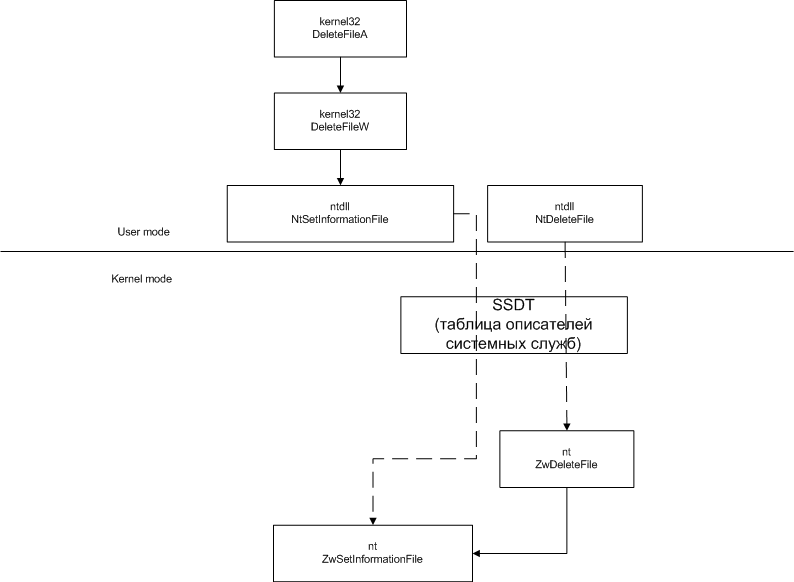
\includegraphics[width=\linewidth]{img/DeleteFileAPIs.png}
	\caption{Функции, отвечающие за удаление файлов}
	\label{fig:filedelete}
\end {figure}
На схеме изображена последовательность вызывающих друг друга функций для реализации удаления. Из неё следует, что в результате запроса об удалении файла ОС всего лишь помечает атрибуты объекта файла на удаление, а само удаление выполняется другим механизмом. Однако, существуют и другие способы удаления файлов. Например, если файл был создан функцией CreateFile с флагом FILE\_FLAG\_DELETE\_ON\_CLOSE, он будет удалён после закрытия все хэндлов и удаления всех ссылок на него без дополнительных обращений из режима пользователя (это пример техники, используемой вирусами для уничтожения следов после осуществеления вредоносной деятельности в системе).
\subparagraph {Создание процессов}
Для создания процессов есть множество различных путей, в том числе, и за рамками приведённых API функций, и нельзя полагаться, что любой создаваемый процесс будет обнаружен, если следить только за ними (рис. \ref{fig:createprocess}).
\begin {figure}[h]
	\centering
	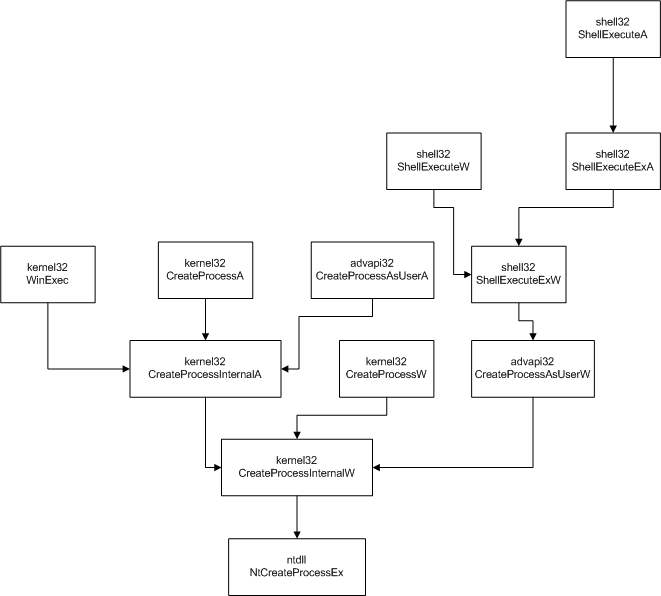
\includegraphics[width=\linewidth]{img/ExampleProcessCreateAPIs.png}
	\caption{Функции, отвечающие за создание процесса}
	\label{fig:createprocess}
\end {figure}
\subsection {Выводы по разделу}
В настоящем разделе был произведён анализ ограничений статических методов исследования исполняемого кода, рассмотрены возможные методы реализации динамического анализа, выбран имеющий наибольшие преимущества и являющийся достаточно простым в реализации вариант, а также проанализированы группы некоторых из Windows API функций, использование которых представляется наиболее значительным при рассмотрении поведения программных средств на наличие подозрительных признаков.
	\clearpage
	\section {Специальный раздел}
В настоящем разделе будут описаны выбранный принцип реализации сбора логов из образцов и построенное для этого окружение. Поскольку хранение и обработку логов нельзя осуществлять на той же ОС, где будут исполняться вирусные образцы, данная деятельность будет осуществляться на специально сконфигурированной для этого ОС - "агенте". Существует два варианта организации работы схемы:
\begin {enumerate}
	\item Используя реальные ПК
	\item Используя виртуальные машины
\end {enumerate}
У варианта с реальным ПК есть свои преимущества, например, исчезает необходимость скрывать исполнение
образца в виртуальной машине, однако такой подход требует дополнительного ПК, и в случае,
если число агентов/ элементов окружения будет необходимо увеличить, нескольких. Восстановление агента
до изначального состояния может быть осуществлено с использованием специализированного ПО (FOG, fogproject.org).

В случае с виртуальными машинами, одного ПК будет достаточно. Однако, во-первых, это потребует дополнительных ресурсов самого ПК, во-вторых, существует множество техник для обнаружения исполнения кода в виртуальной среде, как специфичных для гипервизора, так и общих. Набор примерных техник обнаружения описан в  книге \cite{MALWAREANALYSIS} и может заключаться как в поиске присутствия конкретных имён процессов или ключей реестра, так и простом сканировании памяти на наличие строк "VMWare".  Как описано в статье \cite {VMMYTHS}, создатели гипервизоров разрабатывают ПО таким образом, чтобы уменьшить нагрузку,  необходимую для запуска ОС в виртуальной среде, следовательно, различия в поведении некоторых машинных инструкций в виртуальной среде и в реальной является следствием таковых упрощений реализации (например, VMWare эмулирует чипсет Intel 440BX для всех типов виртуальных машин, поскольку эмуляция всё появляющихся моделей и совместимого с ними оборудования потребовала бы слишком больших затрат и не принесла бы никакой практической с точки зрения производительности пользы). Для проверки возможных способов обнаружения виртуальной машины можно воспользоваться pafish (https://github.com/a0rtega/pafish). Однако, не следует считать наличие таких техник огромным недостатком использования виртуальных машин, т.к. в настоящее время вследствие простоты развёртывания и восстановления использование виртуальной инфраструктуры набирает популярность не только в целях исследования вирусов, но и в обычных организациях. Дальнейшее присутствие таких техник во вредоносном ПО и отказ от исполнения вредоносных действий в случае обнаружения будет наносить вред только лицам, его создающим.

Даже учитывая вышеупомянутые минусы виртуальных машин, всё же, возможность восстановления их до чистого состояния путём использования снапшотов представляется слишком удобной, чтобы обходиться без неё (гипервизор хранит на жёстком диске реального ПК разницу виртуальной оперативной памяти и разницу в секторах виртуального жёсткого диска в виде файлов, и просто восстанавливает файлы до исходного состояния). В качестве виртуальной среды была выбрана Oracle VirtualBox, поддерживающая снапшоты в бесплатной версии по сравнению с аналогичной продукцией от VmWare. Также, используется API VirtualBox для передачи файлов через предоставляемый Oracle модуль-обёртку на Python vboxapi (однако, факт использования данной реализации может быть использован в качестве одной из вышеупомянутых специфичных для VirtualBox техник обнаружения виртуальной машины, т.к. требует установки служб VirtualBox guest additions на агента, и поэтому возможно изменение подхода в дальнейшем). Помимо агента с ОС Windows, на котором будут исполняться исследуемые образцы, также используется виртуальная машина под управлением Debian 8 с установленным на неё пакетом INetSim, который предназначен для эмуляции многих сетевых служб. Поддерживая http, https, ftp, pop3 и многие другие протоколы, INetSim в том числе в состоянии по URL получаемого запроса определять тип файла и посылать в ответ поддельный файл такого же типа (.jpg, .ico, .exe и т.д.). Виртуальная машина с Debian помещается в ту же локальную сеть, что и  исследуемый агент, она же настраивается как сетевой шлюз для него, и одновременно - DNS сервер. Таким образом, на все поддерживаемые INetSim запросы, отправляемые с исследуемого агента на произвольные адреса, будет получен поддельный ответ, что должно позволить собрать больше информации о действиях образцов (например, скачивание и запуск исследуемым образцом поддельного .exe файла от INetSim свидетельствует о поведении, характерном для вредоносного ПО в основном служащего лишь каналом для загрузки другого вредоносного ПО).

По аналогии с последовательностью, описанной в статье \cite {MASSMALWARE}, получена следующая последовательность шагов, представляющая собой цикл исполнения образцов в VirtualBox. Их реализация находится в /vbox/tools/vmrun\_cycled.py

\begin {itemize}
	\item Предварительная конфигурация агента
	\item Загрузка образца
	\item Запуск отслеживающих инструментов и исполнение образца
	\item Получение логов
\end {itemize}

Для ускорения сбора представляется возможным параллельный запуск многих агентов Windows. При этом для каждого из них выполняется указанная последовательность шагов. Фактор ускорения сбора приблизительно равен числу используемых виртуальных машин с Windows. Выделив под основной ПК Intel Xeon e1245v3 (4-core, HyperThreading) и 10 Гб ОЗУ (отдельно для виртуальных машин) удалось добиться комфортной работы параллельно порядка 8--10 агентов Windows. Порядок взаимодействия виртуальных машин при использовании двух агентов Windows и основного ПК приведен на рис. \ref {fig:vmcycle}. При использовании большего числа агентов Windows порядок взаимодействия аналогичен, а ограничения на число агентов зависит в основном только от используемого аппаратного обеспечения.
\begin {figure}[h!]
	\centering
	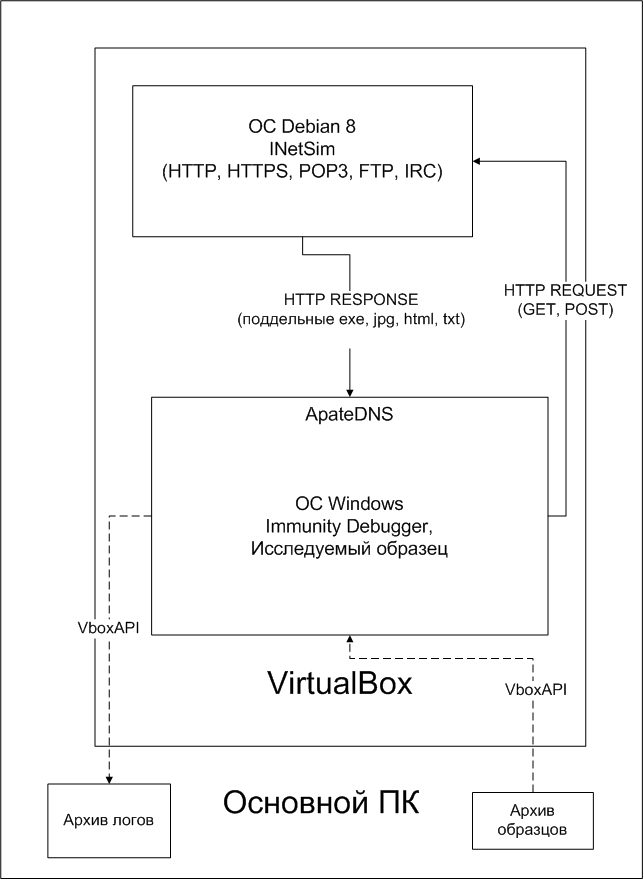
\includegraphics[width=\linewidth] {img/vmcycle.png}
	\caption {Пути взаимодействия компонентов системы сбора логов}
	\label {fig:vmcycle}
\end {figure}

\subsection {Предварительная конфигурация агента}
\subsubsection {Настройка окружения}
Здесь большинство действий было выполнено однократно, после чего был создан снапшот состояния с настроенным окружением, готовым к запуску. Установлен отладчик Immunity Debugger, изменены его настройки, установлен Python 2.7.1, необходимый для работы отладчика, ApateDNS (утилита, позволяющая перенаправлять все DNS запросы на указанный IP адрес), .Net Framework 4.0, 4.5 (некоторые образцы основаны на данной платформе, и иначе запустить их не удастся), выключен файрвол Windows и служба контроля учётных записей (User account control).
Далее на этом шаге просто происходит возврат в "чистое состояние" исследуемого агента и виртуальной машины с INetSim.
\subsubsection {Маскировка виртуальной среды}
Для маскировки исполнения в виртуальной среде были применены следующие модификации виртуальной машины:
\begin {itemize}
	\item Добавлена информация из DMI (Desktop Management Interface)

	DMI позволяет программному обеспечению получать информацию из BIOS, об оборудовании и материнской плате (скопирована с основного ПК с использованием утилиты dmidecode).
	\item Добавлена таблица ACPI (Advanced Configuration and Power Interface)

	ACPI реализует интерфейс для управления питанием и конфигурации материнской платы и устройств. Для этого в оперативной памяти размещается несколько таблиц, содержащих методы управления ими и их описание. При помощи утилиты acpidump с основного ПК была скопирована такая таблица и подключена к виртуальной машине.
	\item Сгенерирован случайный MAC сетевой карты

	По умолчанию присваиваемые MAC адреса относятся к диапазону, начинающемуся с 08-00-27 и могут быть таким образом обнаружены. Взят случайный адрес из диапазона Intel.
	\item Изменена информация об HDD
	\item Изменена информация о CD-приводе
	\item Модифицированы разделы реестра

	Изменены разделы реестра SystemBiosDate, VideoBiosVersion и др., имеющие значение по умолчанию при создании виртуальной машины, позволяющие идентифицировать её как экземпляр VirtualBox.
\end {itemize}
Данный функционал реализуется в рамках vbox/tools/HideVBox/camouflage.py

\subsection {Загрузка образца}
VirtualBox предоставляет доступ к управлению различными функциями виртуальных машин через модуль-обёртку на ЯП Python, названную vboxapi. Используя его, реализован скрипт, скачивающий с основного ПК образец и скрипты, управляющие сбором логов.
\subsection {Запуск отслеживающих инструментов и исполнение образца}
Поскольку снапшоты восстанавливаются из готового состояния, ApateDNS уже запущена и настроена на сервер INetSim.

Образец исполняется в отладчике, после чего специальный скрипт собирает информацию о присутствующих в таблице импортов исполняемого файла функций и устанавливает на них точки останова. Тот же скрипт регистрирует хук, в котором описаны необходимые для получения параметры в случае вызова таковых функций.
В случае вызова функции, отладчик логирует всё в файл. Образец исполняется в течение двух минут.
\subsection {Получение логов}
По истечении указанного промежутка времени скрипт через vboxapi забирает собранные логи о деятельности образца и выключает обе виртуальные машины. После этого происходит выборка из архива следующего образца и запуск следующей итерации цикла для его исследования.

\subsection {Алгоритм сравнения цепочек}
 Для принятия решения о нахождении похожих цепочек вызовов в логах необходимо выбрать способ. Далее будет описан выбранный алгоритм, позволяющий находить не только идентичные цепочки, но и видоизменённые до определённой степени вставленными в них дополнительными вызовами, например:

kernel32.OpenFile -> kernel32.SetFilePointer -> kernel32.Sleep -> kernel32.WriteFile

vs

kernel32.CreateFile -> kernel32.SetFilePointer -> ---  ->   kernel32.WriteFile

Указанные цепочки будут совмещены как похожие, если в матрице цен указать достаточное значение близости OpenFile к CreateFile.
В данном случае пропуск  вызова (символа) при сравнении двух последовательностей будет обозначаться как ``---'', и аналогичен совмещению (kernel32.Sleep, --- ) при выравнивании цепочек.
\subsection {Приведение данных к удобной для обработки форме}
Собранные текстовые логи работы вредоносных образцов являются достаточно информативными с точки зрения ручного анализа, однако для автоматической обработки их следует привести к более компактной и быстрее обрабатываемой форме (как правило, в любых языках программирования операции над строками медленнее операций над числовыми данными). Для анализа цепочек было решено хранить информацию о вызовах как массив из int32 (4 байта на один вызов). Такая форма достаточна для хранения более чем 4 миллионов различных вызовов, а также она поддерживается пакетом numpy ЯП Python. При этом словарь, отображающий эти числа обратно в фактические имена (и, возможно, параметры) функци хранится отдельно. Это позволяет в дальнейшем возвращать более подробную информацию о найденных совпадениях цепочек.

Поскольку размер цепочек произволен, хранение в отдельном файле каждой цепочки потенциально может привести к напрасной трате места хранения на жёстком диске. Например, цепочка длиной в 100 вызовов, занимающая согласно выбранной форме представления 400 байт, будет фактически иметь минимальный размер файла величиной с установленный кластер (обычно 4096 байт). Поэтому для хранения массивов numpy был выбран формат HDF5 (Hierarhical Data Format, иерархический формат данных). Он поддерживает хранение в одном файле некоторого подобия иерархической файловой системы, состоящей из массивов numpy, при этом к каждой отдельной цепочке может быть получен доступ по уникальному имени пути. Это позволяет решить проблему затрат лишнего места на хранение, т.к. теперь как максимум будет потеряно до 4  килобайт на все цепочки целиком. Для работы с файлами такого формата в ЯП Python присутствует модуль h5py.
 Реализация данного преобразования хранится в lib/pander.py.
\subsection {Алгоритм Смита-Ватермана}
Для сравнения как бинарных, так и текстовых строк (или в нашем случае --- последовательности чисел) классической метрикой является расстояние Левенштейна (также называемое дистанцией редактирования). Между двумя строками дистанцией редактирования будет являться число базовых операций, применяемых к одной строке, чтобы получить другую. К базовым операциям относятся:
\begin {itemize}
	\item Вставка одного символа
	\item Удаление одного символа
	\item Замена одного символа на другой
\end {itemize}
Эта  метрика используется в алгоритме Смита-Ватермана, впервые опубликованном в \cite{LOCALALIGNMENT}. Несмотра на то, что придуман он был для нахождения участков похожих цепочек нуклеотидных последовательностей и относится к генетике, можно упомянуть, что некоторые авторы \cite{BLACKBOOK} относятся к проблеме компьютерных вирусов как к искусственной форме жизни (если точнее, то self-replicating automata, "самовоспроизводящийся автоматический механизм"), поэтому идеи ближе, чем может показаться на первый взгляд.

Существует два основных подхода к сравнению последовательностей: глобальное и локальное выравнивание. Применение глобального выравнивания требует примерно одинаковой длины цепочек, что нельзя гарантировать в случае исследования произвольных образцов. Использование глобального выравнивания можно было бы отнести к поиску практически идентичных копий вредоносных образцов. Алгоритм Смита-Ватермана применяет локальное выравнивание, что ближе к идее нахождения каких-либо распространённых сходных отрезков последовательностей вызовов функций API, потенциально обладающих вредоносным воздействием. Он берёт две последовательности произвольной длины и находит оптимальное выравнивание в любом месте последовательности согласно задаваемой матрице цен, определяющей изменение счёта текущего выравнивания. 

Набор шагов алгоритма для строк $A = a_1 a_2 a_3 ... a_n$ , $B = b_1 b_2 b_3 ... b_m$ длины n и m соответственно заключается в следующем:
\begin {enumerate}
	\item Вычисляем матрицу выравниваний
	Двумерная матрица размерностью в ( n X m) инициализируется нулями. В случае использования локального выравнивания первый столбец и первая строка остаются равными 0, чтобы позволить новому выравниванию начаться в любом месте строки без штрафа за вставку первоначальных символов, идущих до выравнивания. Далее матрица продолжает заполняться слева направо и сверху вниз, при этом каждое новое значение выбирается как максимальное из трёх вариантов:
	\begin {itemize}
		\item Цена совмещения очередного символа первой и второй строки $(a_i, b_j)$ плюс цена, стоящая в матрице выравнивания сверху слева по диагонали (предыдущая цена совмещения двух предыдущих символов строк).
		\item Цена вставки символа первой строки (аналогична совмещению $(a_i, -)$), при этом т.к. не произошло продвижения по символам второй строки, добавляется цена из ячейки, находящаяся сверху от текущей.
		\item Цена вставки символа второй строки (аналогична совмещению $(-, b_j)$), при этом т.к. не произошло продвижения по символам первой строки, добавляется цена, расположенная в матрице слева от вычисляемой ячейки.
	\end {itemize}
	Если получаемое при выборе максимума число отрицательное, вместо него записывается 0, чтобы данная ячейка массива не влияла на нахождение возможных последующих локальных выравниваний.
	После завершения операций матрица выравниваний готова.
	\item Вычисление локального выравнивания

	Задача заключается в обходе матрицы выравниваний по определённым правилам:
	\begin {itemize}
		\item На первом шаге находится максимальное значение цены в матрице и запоминаются индексы позиции (i, j), на которой он располагается
		\item Далее с позицией максимума сравниваются ячейки, стоящие выше, слева и по диагонали от неё, чтобы понять, каким из 3х путей этой ячейке было присвоено значение, соответственно производится уменьшение индекса i, j или обоих сразу, реконструируется часть строки выравнивания, после чего операция повторяется
		\item В случае, если значение ячейки, на которую указывают текущие значения индексов (i, j) равно 0, алгоритм завершает работу, возвращая пару реконструированных строк и счёт оптимального выравнивания
	\end {itemize}
	При необходимости алгоритм можно модифицировать для нахождения нескольких пар выравниваний со значениями меньше, чем у оптимального.
\end {enumerate}
В текущей реализации матрица весов модифицирована следующим образом: вручную указан набор функций, обладающих малой информативностью и при их совмещении добавляется цена 0, также был выбран определённый набор критичных функций, для которых оценка при совпадении вызовов несколько выше, чем для остальных. Для лучшей точности работы следует выдавать близкие оценки функциям, имеющим сходные наборы аргументов и/ или близких по реализуемому ими функционалу (по крайней мере, ASCII/Unicode версиям функций плюс их обычным и Ex вариантам).

Наибольшую трудоёмкость данного алгоритма составляет шаг построения матрицы выравниваний. Если считать, что в среднем длина двух сравниваемых цепочек одинакова, и приняв за n длину цепочки, асимптотическая оценка функции роста данного алгоритма составляет $O(n^2)$. В связи с этим, было принято решение ускорить реализацию данного шага. Это было произведено в рамках использования Cython. Cython - отдельный диалект ЯП Python, позволяющий получить значительное ускорение выполнения трудоёмкого кода через создание расширения, которое будет преобразовано к ЯП C и скомпилировано.  Значительного прироста скорости исполнения можно добиться, всего лишь статически типизировав переменные. После компиляции данное расширение может быть импортировано в обычный Python и использовано без каких-либо дополнительных ограничений. Cython-расширение реализовано в рамках lib/seq\_analyzer/scoring/compare\_samples.pyx.

После применения преобразования в файл hdf5 логов и сохранения полученный набор последовательностей может  быть в любой момент вновь пропущен через алгоритм на новых образцах. 
Алгоритм локального выравнивания реализован в lib/seq\_analyzer/local\_alignment.py
	\clearpage
	\section {Организация процесса сбора данных}
Здесь будут описаны принцип реализации сбора логов из образцов и построенное окружение. Поскольку
хранение и обработку логов нельзя осуществлять на той же ОС, где будут исполняться вирусные образцы,
данная деятельность будет осуществляться на специально сконфигурированной для этого ОС - "агенте". Существует два варианта организации работы схемы:
\begin {enumerate}
	\item Используя реальные ПК
	\item Используя виртуальные машины
\end {enumerate}
У варианта с реальным ПК есть свои преимущества, например, исчезает необходимость скрывать исполнение
образца в виртуальной машине, однако такой подход требует дополнительного ПК, и в случае,
если число агентов/ элементов окружения будет необходимо увеличить, нескольких. Восстановление агента
до изначального состояния может быть осуществлено с использованием специализированного ПО (FOG, fogproject.org).

В случае с виртуальными машинами, одного ПК будет достаточно. Однако, во-первых, это потребует дополнительных ресурсов самого ПК, во-вторых, существует множество техник для обнаружения исполнения кода в виртуальной среде, как специфичных для гипервизора, так и общих. Набор примерных техник обнаружения описан в  книге \cite{MALWAREANALYSIS} и может заключаться как в поиске присутствия конкретных имён процессов/ ключов реестра, так и простом сканировании памяти на наличие строк "VMWare".  Как описано в статье \cite {VMMYTHS}, создатели гипервизоров разрабатывают ПО таким образом, чтобы уменьшить нагрузку,  необходимую для запуска ОС в виртуальной среде, следовательно, различное поведение некоторых машинных инструкций в виртуальной среде и в реальной является следствием таковых упрощений реализации (например, VMWare эмулирует чипсет Intel 440BX для всех типов виртуальных машин, поскольку эмуляция всё появляющихся моделей и совместимого с ними оборудования нетривиальна). Для проверки возможных способов обнаружения виртуальной машины можно воспользоваться pafish (https://github.com/a0rtega/pafish). Однако, не следует считать наличие таких техник огромным недостатком использования виртуальных машин, т.к. в настоящее время вследствие простоты развёртывания и восстановления использование виртуальной инфраструктуры набирает популярность не только в целях исследования вирусов, но и в обычных организациях. Дальнейшее присутствие таких техник во вредоносном ПО будет наносить вред только лицам, его создающим.

Даже учитывая вышеупомянутые минусы виртуальных машин, всё же, возможность восстановления их до чистого состояния путём использования снапшотов представляется слишком удобной, чтобы обходиться без неё (гипервизор хранит на жёстком диске реального ПК разницу виртуальной оперативной памяти и разницу в секторах виртуального жёсткого диска в виде файлов, и просто восстанавливает файлы до исходного состояния). В качестве виртуальной среды была выбрана Oracle VirtualBox, поддерживающая снапшоты в бесплатной версии по сравнению с аналогичной продукцией от VmWare. Также, используется API VirtualBox для передачи файлов через предоставляемый Oracle модуль-обёртку на Python vboxapi (однако, факт использования данной реализации может быть использован в качестве одной из вышеупомянутых специфичных для VirtualBox техник обнаружения виртуальной машины, т.к. требует установки служб VirtualBox guest additions на агента, и поэтому возможно изменение подхода в дальнейшем). Помимо агента с ОС Windows, на котором будут исполняться исследуемые образцы, также используется виртуальная машина под управлением Debian 8 с установленным на неё пакетом INetSim, который предназначен для эмуляции многих сетевых служб. Поддерживая http, https, ftp, pop3 и многие другие протоколы, INetSim в том числе в состоянии по URL получаемого запроса определять тип файла и посылать в ответ поддельный файл такого же типа (.jpg, .ico, .exe и т.д.). Виртуальная машина с Debian помещается в одну локальную сеть с исследуемым агентом, она же настраивается как сетевой шлюз для него, и одновременно - DNS сервер. Таким образом, на все поддерживаемые INetSim запросы, отправляемые с исследуемого агента на произвольные адреса, будет получен муляж ожидаемого ответа, что должно позволить собрать больше информации о действиях образцов (например, скачивание и запуск исследуемым образцом поддельного .exe файла от INetSim свидетельствует о поведении, характерном для вредоносного ПО в основном служащего лишь каналом для загрузки другого вредоносного ПО).

По аналогии с последовательностью, описанной в статье \cite {MASSMALWARE}, получена следующая последовательность шагов, представляющая собой цикл исполнения образцов в VirtualBox. Их реализация находится в /vbox/tools/vmrun\_cycled.py

\begin {itemize}
	\item Предварительная конфигурация агента
	\item Загрузка образца
	\item Запуск отслеживающих инструментов и исполнение образца
	\item Получение логов
\end {itemize}

Порядок взаимодействия виртуальных машин и основного ПК приведена на рис. \ref {fig:vmcycle}
\begin {figure}[h!]
	\centering
	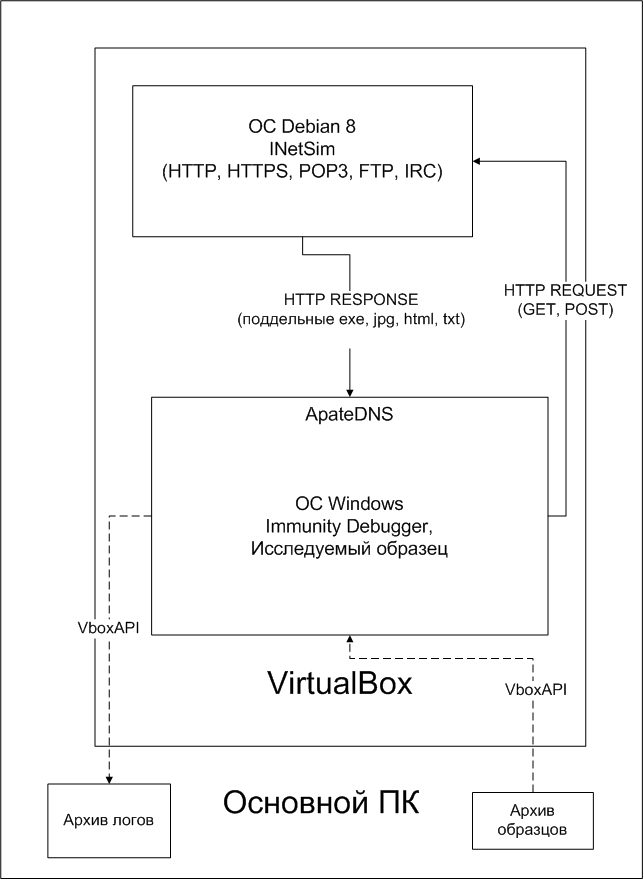
\includegraphics[width=\linewidth] {img/vmcycle.png}
	\caption {Пути взаимодействия компонентов системы сбора логов}
	\label {fig:vmcycle}
\end {figure}

\subsection {Предварительная конфигурация агента}
\subsubsection {Настройка окружения}
Здесь большинство действий было выполнено однократно, после чего был создан снапшот состояния с настроенным окружением, готового к запуску. Установлен отладчик Immunity Debugger, изменены его настройки, установлен Python 2.7.1, необходимый для работы отладчика, ApateDNS (утилита, позволяющая перенаправлять все DNS запросы на указанный IP адрес), .Net Framework 4.0, 4.5 (некоторые образцы построены с его использованием и не работают без него), выключен файрвол Windows и служба контроля учётных записей (User account control).
Далее на этом шаге просто происходит возврат в "чистое состояние" исследуемого агента и виртуальной машины с INetSim.
\subsubsection {Маскировка виртуальной среды}
Для маскировки исполнения в виртуальной среде были применены следующие модификации виртуальной машины:
\begin {itemize}
	\item Добавлена информация из DMI (Desktop Management Interface)

	DMI позволяет программному обеспечению получать информацию из BIOS, об оборудовании и материнской плате (скопирована с основного ПК с использованием утилиты dmidecode).
	\item Добавлена таблица ACPI (Advanced Configuration and Power Interface)

	ACPI реализует интерфейс для управления питанием и конфигурации материнской платы и устройств. Для этого в оперативной памяти размещается несколько таблиц, содержащих методы управления ими и их описание. При помощи утилиты acpidump с основного ПК была скопирована такая таблица и подключена к виртуальной машине.
	\item Сгенерирован случайный MAC сетевой карты

	По умолчанию присваиваемые MAC адреса относятся к диапазону, начинающемуся с 08-00-27 и могут быть таким образом обнаружены. Взят случайный адрес из диапазона Intel.
	\item Изменена информация об HDD
	\item Изменена информация о CD-приводе
	\item Модифицированы разделы реестра

	Изменены разделы реестра SystemBiosDate, VideoBiosVersion и др., имеющие значение по умолчанию при создании виртуальной машины, позволяющие идентифицировать её как экземпляр VirtualBox.
\end {itemize}
Данный функционал реализуется в рамках vbox/tools/HideVBox/camouflage.py

\subsection {Загрузка образца}
Используя vboxapi, реализован скрипт, скачивающий с основного ПК образец и скрипты, управляющие сбором логов.
\subsection {Запуск отслеживающих инструментов и исполнение образца}
Поскольку снапшот восстанавливаются из готового состояния, ApateDNS уже запущена и настроена на сервер INetSim.

Образец исполняется в отладчике, после чего специальный скрипт собирает информацию о присутствующих в таблице импортов исполняемого файла функций и устанавливает на них точки останова. Тот же скрипт регистрирует хук, в котором описаны необходимые для получения параметры в случае вызова таковых функций.
В случае вызова функции, отладчик логирует всё в файл. Образец исполняется в течение 2 мин.
\subsection {Получение логов}
По истечении указанного промежутка времени скрипт через vboxapi забирает собранные логи о деятельности образца и выключает обе виртуальные машины. После этого происходит выборка из архива следующего образца и запуск следующей итерации цикла для его исследования.



 

	\clearpage
           \section {Экономический раздел}
\subsection {Планирование разработки программного продукта с построением графика}
В дипломном проекте производится «Разработка программного модуля анализа защищённости СВТ от ВПО». В данном разделе определяется трудоемкость и затраты на создание ПО, а также производится расчет времени, необходимого для создания базы знаний, необходимой для работы программного средства в рамках испытания. 
\subsubsection {Определение трудоемкости и продолжительности работ по разработке программного модуля анализа защищённости СВТ от ВПО.}
Процесс разработки включает: обзор и анализ программных средств схожей тематики, анализ и выбор программных продуктов для создания программы; отладка; испытание. В свою очередь каждый из этих этапов можно подразделить на отдельные подэтапы.
Согласно ГОСТ 23501.1-79 регламентируются следующие стадии проведения исследования:
\begin {itemize}
	\item техническое задание – ТЗ (ГОСТ 23501.2-79);
	\item эскизный проект – ЭП (ГОСТ 23501.5-80);
	\item технический проект – ТП (ГОСТ 23501.6-80);
	\item рабочий проект – РП (ГОСТ 23501.11-81);
	\item внедрение – ВП (ГОСТ 23501.15-81).
\end {itemize}

Планирование стадий и содержания работ осуществляется в соответствии с \cite {ECONOMICS}. На всех стадиях проведения исследования выполняются следующие виды работ, перечень которых показан в таблице \ref {table:joblist}.

\begin{table}
	\begin {tabular}{|p{10em}|p{20em}|}
	\hline
	Стадии разработки & Перечень работ \\ \hline
	Техническое задание & -- постановка задачи; \\
	&  -- подбор литературы; \\
	& -- сбор исходных данных; \\
	& -- определение требований к системе; \\
	& -- определение стадий, этапов и сроков разработки ПО;\\ \hline
	Эскизный проект & -- анализ программных средств схожей тематики; \\
	&  -- разработка общей структуры ПО; \\
	& -- разработка структуры программы по подсистемам; \\
	& -- документирование; \\ \hline
	Технический проект & -- определение требований к ПО; \\
	&  -- выбор инструментальных средств; \\
	& -- определение свойств и требований к аппаратному обеспечению; \\ \hline
	Рабочий проект & -- верстка и дизайн; \\
	&  -- программирование; \\
	& -- тестирование и отладка ПО; \\
	& -- разработка программной документации; \\
	& -- согласование и утверждение работоспособности системы; \\ \hline
	Внедрение & -- опытная эксплуатация; \\
	&  -- программирование; \\
	& -- анализ данных, полученных в результате эксплуатации; \\
	& -- корректировка технической документации по результатам испытаний; \\ \hline
	\end {tabular}
	\caption{Перечень работ на каждой стадии проведения исследования}
	\label{table:joblist}
\end{table}

Трудоемкость выполнения работ по созданию ПО на каждой из стадий определяется в соответствии с \cite {ECONOMICSSECTION} и \cite {ECONOMICSDIPLOMA}.

Трудоемкость выполнения работ по созданию ПО определяется по сумме трудоемкости этапов и видов работ, оцениваемых экспертным путем в человеко-днях, и носит вероятностный характер, так как зависит от множества трудно учитываемых факторов.

Трудоемкость каждого вида работ определяется по формуле \eqref {eq:worksize}.
\begin {equation}
    \label {eq:worksize}
    t_i = \frac {3 * t_{min} + 2 * t_{max}}{5},
\end {equation}
где:

$t_{min}$ – минимально возможная трудоемкость выполнения отдельного вида работ;

$t_{max}$ – максимально возможная трудоемкость выполнения отдельного вида работ.

Продолжительность каждого вида работ в календарных днях ($T_i$) определяется по формуле \eqref {eq:calendarwork}, в днях:
\begin {equation}
    \label {eq:calendarwork}
    T_i = \frac {t_i}{\text{Ч}_i} * K_\textup{вых},
\end {equation}
где:

$t_i$ – трудоемкость работ, человек-дней;

$\text{Ч}_i$ – численность исполнителей, человек;

$K_\textup{вых}$ – коэффициент, учитывающий выходные и праздничные дни:
\begin {equation*}
    K_\textup{вых} = \frac {K_\textup{кал.}}{K_\textup{раб.}},
\end {equation*}	 
где:

$K_\textup{кал}$ – число календарных дней;

$K_\textup{раб.}$ – рабочие дни;

$K_\textup{вых}=1,3$.

Полный список видов и этапов работ по созданию ПО, экспертные оценки и расчетные величины их трудоемкости, а также продолжительность каждого вида работ, рассчитанные по формулам \eqref{eq:worksize} и \eqref{eq:calendarwork}, представлены в таблице \ref {table:worklength}

\begin{longtable}{| p{2em}|>{\raggedright\arraybackslash}p{12em}|p{2em}|p{2em}|p{2em}|p{2em}|p{5em}|}
	\caption{Расчёт трудоёмкости и продолжительности работ по созданию ПО}\\ \hline
	\label{table:worklength}
	\rotatebox[origin=c]{90}{№ работы} & Стадии разработки & \multicolumn{3}{|p{6em}|}{\rotatebox[origin=c]{90}{Трудоёмкость, чел.дни}} & \rotatebox[origin=c]{90}{Количество работников} & \rotatebox[origin=c]{90}{\parbox{8em}{Продолжительность работ, \\ календарные дни}} \\ \cline{3-7}
	& & $t_{min}$ & $t_{max}$ & $t_i$ & $\text{Ч}_i$ & $T_i$  \endfirsthead 
	\multicolumn{7}{c}{{\tablename\ \thetable{} -- продолжение}} \\ \hline
	1 & 2 & 3 & 4 & 5 & 6 & 7\endhead\hline
	1 & 2 & 3 & 4 & 5 & 6 & 7\\ \hline
	\multicolumn{7}{|c|}{Техническое задание} \\ \hline
	1 & - постановка задачи & 2 & 2 & 2 & 1 & 2.6 \\ \hline
	2 & - подбор литературы & 4 & 7 & 5.2 & 1 & 6.8 \\ \hline
	3 & - сбор исходных данных & 8 & 12 & 9.6 & 1 & 12.5\\ \hline
	4 & - определение требований к системе & 1 & 2 & 1.4 & 1 & 1.8\\ \hline
	5 & - определение стадий, этапов и сроков разработки ПО & 2 & 3 & 2.4 & 1 & 3.1\\ \hline
	\multicolumn{7}{|c|}{Эскизный проект}\\ \hline
	6 & - анализ программных средств схожей тематики & 7 & 8 & 7.4 & 1 & 9.6\\ \hline
	7 & - разработка общей структуры ПО & 3 & 5 & 3.8 & 1 & 4.9\\ \hline
	8 & - разработка структуры программы по подсистемам & 4 & 6 & 4.8 & 1 & 	6.2\\ \hline
	9 & - документирование & 1 & 3 & 1.8 & 1 & 2.3\\ \hline
	\multicolumn{7}{|c|}{Технический проект}\\ \hline
	10 & - определение требований к ПО	& 1 & 2 & 1.4 & 1 & 1.8\\ \hline
	11 & - выбор инструментальных средств & 1 & 1 & 1 & 1 & 1,3\\ \hline
	12 & - определение свойств и требований  к аппаратному обеспечению & 1 & 1 & 1 & 1 & 1.3\\ \hline
	\multicolumn{7}{|c|}{Рабочий проект}\\ \hline
	13 & - дизайн проекта & 2 & 4 & 2.8 & 1 & 3.6\\ \hline
	14 & - программирование & 8 & 12 & 9.6 & 1 & 12.5\\ \hline
	15 & - тестирование и отладка ПО & 20 & 25 & 22 & 1 & 28.6\\ \hline
	16 & - разработка программной документации & 3 & 5 & 4.8 & 1 & 6.2\\ \hline
	17 & - согласование и утверждение работоспособности системы & 2 & 3 & 2.4 & 1 & 3.1\\ \hline
	\multicolumn{7}{|c|}{Внедрение}\\ \hline
	18 & - опытная эксплуатация & 11 & 22 & 15.4 & 1 & 20\\ \hline
	19 & - анализ данных, полученных в результате эксплуатации & 3 & 4 & 3.4 & 1 & 4.4\\ \hline
	20 & - корректировка технической документации по результатам испытаний & 1 & 2 & 1.4 & 1 & 1.8\\ \hline
	& \textbf{Общая трудоёмкость разработки} & & & \textbf{104} & & \textbf{134}\\ \hline
\end{longtable}
Таким образом, общая продолжительность проведения работ составит 134 календарных дней.

\subsubsection {Построение ленточного графика проведения исследования}
В качестве инструмента планирования работ используем ленточный график. Ленточный график позволяет наглядно представить логическую последовательность и взаимосвязь отдельных работ, срок начала и срок окончания работ. Он представляет собой таблицу, где перечислены наименования стадий разработки и видов работ, длительность выполнения каждого вида работ. Продолжением таблицы является график, отражающий продолжительность каждого вида работ в виде отрезков времени, которые располагаются в соответствии с последовательностью выполнения работ. 

Ленточный график разработки ПО, построенный по данным таблицы \ref {table:worklength}, приведен на рисунке \ref {fig:workflow}.

\begin {figure}
	\centering
	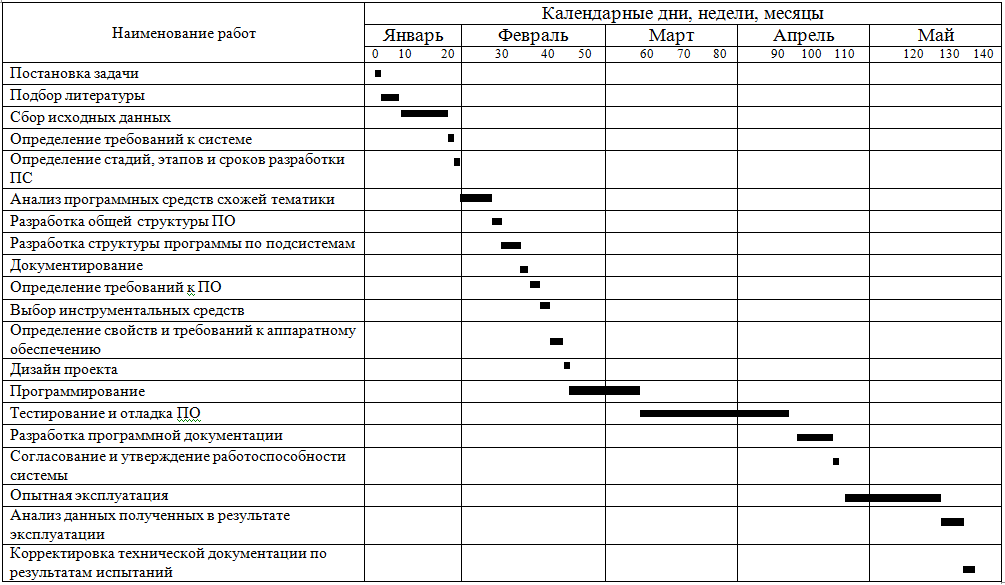
\includegraphics[angle=90,scale=0.95]{img/WorkFlow.png}
	\caption{Ленточный график разработки ПО}
	\label{fig:workflow}
\end {figure}

\subsection {Расчёт сметы затрат на разработку программного продукта}

Сметная стоимость проектирования и внедрения программы включает в себя следующие затраты, определяемые по формуле \eqref{eq:project}:
\begin {equation}
    \label {eq:project}
    C_\textup{пр}=C_\textup{осн} + C_\textup{доп} + C_\textup{соц} + C_\textup{м} + C_\textup{маш},
\end {equation}

где

$C_\textup{пр}$ – стоимость разработки ПО;

$C_\textup{осн}$ – основная заработная плата исполнителей;

$C_\textup{доп}$ – дополнительная заработная плата исполнителей, учитывающая потери времени на отпуска и болезни (принимается в среднем 10\% от основной заработной платы);

$C_\textup{соц}$ – отчисления во внебюджетные фонды государственного социального страхования (пенсионный фонд, фонд обязательного медицинского страхования, фонд социального страхования), рассчитываются как 30,2\% от основной и дополнительной заработной платы;

$C_\textup{м}$ – затраты на используемые материалы;

$C_\textup{маш.вр}$ – стоимость машинного времени.

$C_\textup{н}$ – накладные расходы включают затраты на управление, уборку, ремонт, электроэнергию, отопление и др. (принимаются в размере 60\% от основной и дополнительной заработной платы);

\begin {center}
	\textbf{Основная заработная плата исполнителей.}
\end {center}

На статью «Заработная плата» относят заработную плату научных, инженерно-технических и других работников, непосредственно участвующих в разработке ПО. Расчет ведётся по формуле \eqref {eq:executer_salary}:
\begin {equation}
    \label{eq:executer_salary}
    \text{З}_\textup{исп} = \text{З}_\textup{ср} *\text{Т},
\end {equation}

где

$\text{З}_\textup{исп}$ – заработная плата исполнителей (руб.);

$\text{З}_\textup{ср}$ – средняя тарифная ставка работника организации разработчика ПО (руб./чел./дни);

$\text{Т}$ – трудоемкость разработки ПО (чел.дни).

$\text{З}_\textup{ср}$ определяется по формуле \eqref {eq:average_salary}:
\begin {equation}
    \label {eq:average_salary}
    \text{З}_\textup{ср} = \text{С} / \text{Ф}_\textup{мес},
\end {equation}
где

$\text{С}$ – зарплата труда на текущий момент времени (руб./мес.);

$\text{Ф}_\textup{мес}$ – месячный фонд рабочего времени исполнителя (дни).

Затраты на статью «Заработной платы» приведены в таблице \ref{table:cost_salary}.

\begin{table}[h]
	\begin {tabular}{|p{2em}|p{6em}|p{4em}|p{6em}|p{7em}|p{6em}|}
		\hline
		№ & Исполнитель & Оклад, руб./мес. & Оклад., руб./день & Трудоемкость, чел.дни & Сумма, руб.\\ \hline
		1 & Инженер-программист & 60000 & 2000 & 104 & 208000 \\ \hline
		\multicolumn{4}{|p{16em}|}{Общая основная зарплата исполнителей, $C_\textup{осн}$} & 104 & 208000\\ \hline
	\end {tabular}
	\caption{Затраты на заработную плату}
	\label{table:cost_salary}
\end{table}

\begin {center}
	\textbf{Дополнительная заработная плата}
\end {center}

Дополнительная заработная плата на период разработки ПО рассчитывается относительно основной и составляет 10\% от ее величины:
\begin {equation}
                                  C_\textup{доп} = C_\textup{осн} * 0,1 = 20800 (\text{руб.})
\end {equation}

\begin {center}
	\textbf{Расчет отчислений на социальное страхование}
\end {center}

Социальное страхование включает отчисления во все внебюджетные фонды, в том числе пенсионный, занятости, обязательного медицинского страхования, социального страхования. Отчисления на социальное страхование рассчитываются относительно выплаченной заработной платы (суммы основной и дополнительной заработной платы). Составляют 30,2\%:
\begin {equation}
                          C_\textup{соц} = (C_\textup{осн} + C_\textup{доп}) * 0,302
\end {equation}
\begin {equation*}
	C_\textup{соц} = (208000 + 20800) * 0,302 = 69097.6 (\text{руб.})
\end {equation*}

\begin {center}
	\textbf{Расчет расходов на материалы}
\end {center}

На эту статью относят все затраты на магнитные носители данных, бумагу, для печатных устройств, канцтовары и др. Затраты по ним определяются по экспертным оценкам. Расчет расходов на материалы приведен в таблице \ref{table:cost_materials}.

\begin{table}
	\begin {tabular}{|p{3em}|p{10em}|p{8em}|p{8em}|}
		\hline
		№ & Материалы & Количество, штуки & Стоимость, рубли\\ \hline
		1 & Бумага писчая, листов & 1000 & 400 \\ \hline
		2 & Картридж для принтера, шт. & 1 & 900\\ \hline
		3 & HDD Seagate Constellation ES.3 ST3000NM0033 для виртуальных машин/архивов с ВПО & 1 & 10746\\ \hline
		\multicolumn{3}{|p{21em}|}{Общая стоимость материалов, $C_\textup{м}$} & 12046\\ \hline
	\end {tabular}
	\caption{Стоимость материалов}
	\label{table:cost_materials}
\end{table}

\begin {center}
	\textbf{Накладные расходы}
\end {center}

На статью «Накладные расходы» относят расходы, связанные с управлением и организацией работ. Накладные расходы рассчитываются относительно основной заработной платы. Величина накладных расходов принимается равной 60\% от основной зарплаты исполнителей. Формула расчёта \eqref{eq:overhead_cost}:
\begin {equation}
    \label {eq:overhead_cost}
    C_\textup{н} = C_\textup{осн} * \text{К}
\end {equation}
где

$C_\textup{н}$ – накладные расходы (руб.);

$C_\textup{осн}$ – основная заработная плата исполнителей (руб.);
$\text{К}$ – коэффициент учета накладных расходов ($\text{К} = 0,6$)
\begin {equation*}
    C_\textup{н} = 208000 * 0,6 = 124800 (\text{руб.})
\end {equation*}

\begin {center}
	\textbf{Расчет стоимости машинного времени}
\end {center}

Затраты на машинное время, необходимое для разработки ПО, расходы на приобретение и подготовку материалов научно-технической информации, расходы на использование средствами связи. Расчет затрат на машинное время осуществляется по формуле \eqref{eq:computer_time}:
\begin {equation}
    \label{eq:computer_time}
    C_\textup{маш.вр} = \text{К}_\textup{маш.вр} * \text{З}_\textup{маш.вр}
\end {equation}

где
$\text{К}_\textup{маш.вр}$ – тарифная стоимость одного часа машинного времени ($\text{К}_\textup{маш.вр}=50 \text{руб./ч.}$)

Тарифная стоимость 1 суток работы составляет:
\begin {equation*}
    C_\textup{cуток} = 24 * \text{К}_\textup{маш.вр} = 24 * 50 = 1200 (\text{руб.})
\end {equation*}

$\text{З}_\textup{маш.вр}$ – машинное время, используемое на проведение работ.

Необходимое количество машинного времени для реализации проекта по разработке программы рассчитывается по формуле \eqref {eq:impl_time}:
\begin {equation}
    \label {eq:impl_time}
    \text{З}_\textup{маш.вр} = t_i * T_\textup{см} * T_\textup{ср.маш},
\end {equation}

где

$t_i$ – трудоемкость работ, чел.дней;

$T_\textup{см}$ – продолжительность рабочей смены (при пятидневной рабочей неделе $T\textup{см} = 8 \text{ч.}$);

$T\textup{ср.маш}$ – средний коэффициент использования машинного времени ($T\textup{ср.маш} = 0,7$).

Тогда:
\begin {equation*}
    \text{З}_\textup{маш.вр} = 104 * 8 * 0,7 = 582 (\text{ч.})
\end {equation*}

Стоимость машинного времени составит:
\begin {equation*}
    C_\textup{маш.вр} = 50 * 582 = 29100 (\text{руб.})
\end {equation*}

Результаты расчета затрат на проектирование программного обеспечения сведены в таблице \ref{table:cost_outlay}.
\begin{table}[h]
	\begin {tabular}{|p{3em}|p{10em}|p{6em}|p{6em}|p{6em}|}
		\hline
		№ & Наименование статей & Обозначение & Сумма, руб. & В \% к итогу\\ \hline
		1 & 2 & 3 & 4 & 5 \\ \hline
		1 & Основная заработная плата & $C_\textup{осн}$ & 208000 & 44.84 \\ \hline
		2 & Дополнительная заработная плата & $C_\textup{доп}$ & 20800 & 4.48\\ \hline
		3 & Отчисления на социальные нужды & $C_\textup{соц}$ & 69097.6 & 14.9\\ \hline
		4 & Материалы & $C\textup{мат}$ & 12046 & 2.6\\ \hline
		5 & Стоимость машинного времени & $C\textup{маш.вр.}$ & 29100 & 6.27\\ \hline
		6 & Накладные расходы & $C\textup{н}$ & 124800 & 26.9\\ \hline
		\multicolumn{2}{|p{13em}|}{Итого:} & $C\textup{пр}$ & 463843.6 & 100\\ \hline
	\end {tabular}
	\caption{Смета затрат на разработку и внедрение программы}
	\label{table:cost_outlay}
\end{table}

Таким образом, себестоимость разработки составляет \textbf{463843.6} руб.

Данная программа может быть реализована на рынке. При расчетном количестве реализованных программ (n=100), оптовая цена программы ($\text{Ц}_\textup{опт}$) может быть рассчитана по формуле \eqref {eq:wholesale}:
\begin {equation}
    \label {eq:wholesale}
    \text{Ц}_\textup{опт} =  \frac{C_\textup{пр}}{n} + \text{П} ;
\end {equation}
где

$C\textup{пр}$ – себестоимость разработки программы;

П – прибыль, определяется по формуле \eqref {eq:gains}:
\begin {equation}
    \label {eq:gains}
    \text{П}_i = \text{Ур} * \frac{C_\textup{пр}}{n} * 100,
\end {equation}
где

$\text{Ур}$ – средний уровень рентабельности ($\text{Ур} = 20\%$).

Таким образом, оптовая цена программы составит:
\begin {equation*}
\text{Ц}_\textup{опт} = 463843.6/100 + (463843.6/100)*0.2 = \textbf{5566.1} (\text{руб.})
\end {equation*}
Отпускная цена реализации программы потребителям (Цотп), рассчитывается по формуле \eqref {eq:saleprice}:
\begin {equation}
    \label {eq:saleprice}
    \text{Ц}_\textup{отп} = \text{Ц}_\textup{опт} + \text{НДС},
\end {equation}
где

НДС – налог на добавленную стоимость, рассчитывается в соответствии с действующей ставкой этого налога – 18\% от оптовой цены программы.
\begin {equation*}
    \text{Ц}_\textup{отп}  = 5566.1 + 5566.1*0.18 = 5566.1 + 1001,9 = \textbf{6568} (\text{руб.})
\end {equation*}

Таким образом, отпускная цена программы составит \textbf{6568}  руб., в том числе НДС – \textbf{1001,9}  руб.

\subsection {Расчёт основных технико-экономических показателей и эффективности использования программного продукта}
В настоящей дипломной работе проведена программная реализация алгоритмов, направленных на обнаружение похожего поведения вредоносного ПО, а также собран один из вариантов сред, используемых для исследования их поведения. При увеличении машинного времени, выделяемого для сбора цепочек на известных образцах ВПО, точность обнаружения потенциально неизвестных вирусов будет увеличена (т.к. скорость прогона образцов на данном хосте за сутки составляет около 6000 шт./сутки, за каждые $C_\textup{cуток} = 1200 \text{руб.}$ возможно  увеличение числа собранных цепочке на соответствующее число). 

Также предусматривается возможность доработки программного продукта в рамках использования других сред виртуализации. Это приведёт  к более эффективному использованию аппаратного обеспечения, на котором собираются цепочки вызовов ВПО на предоставляемых программе образцах, и, возможно, позволит увеличить число параллельно работающих виртуальных машин. Всё это предоставляет возможности для обнаружения новых вредоносных программ, имеющих подозрительное поведение.

\begin{longtable}{| >{\centering\arraybackslash}p{10em}|>{\centering\arraybackslash}p{6em}|>{\centering\arraybackslash}p{12em}|}
	\caption{Основные технико-экономические показатели проекта}\\ \hline
	\label{table:project_tth}
	Наименование показателя & Ед. измерения & Проектный вариант\endfirsthead
	\multicolumn{3}{c}{{\tablename\ \thetable{} -- продолжение}} \\ \hline
	1 & 2 & 3\endhead \hline
	1 & 2 & 3\\ \hline
	Способ обработки информации& --- & С применением ЭВМ и програмных средств \\ \hline
           Характеристики исследования: & & \\ \hline
	Язык программирования & --- & CPython 3.4\\ \hline
	Использованные технические средства: & &\\ \hline
	Хост для запуска виртуальных машин & --- & Intel Xeon E3-1245v3, 4 x 8Gb DDR1600, HDD 3 Tb/7200/64Mb, int. Video, LAN, ATX 1000W\\ \hline
	Принтер & --- & HP LaserJet 6L\\ \hline
	Количество исследователей & чел & 1\\ \hline
	Продолжительность проведения исследования & календарных дней & 134\\ \hline
	Трудоёмкость проведения исследования & чел-дней & 104\\ \hline
	Затраты на проведение исследования & руб. & 463843.6\\ \hline
	в том числе: &  & \\ \hline
	Стоимость расходных материалов & руб. & 12046\\ \hline
	Основная заработная плата & руб. & 208000\\ \hline
	Дополнительная заработная плата & руб. & 20800\\ \hline
	Отчисления на социальные нужды & руб. & 69097.6\\ \hline
	Накладные расходы & руб. & 124800\\ \hline
	Стоимость машинного времени & руб. & 29100\\ \hline
\end{longtable}


	\clearpage
           \section {Экономический раздел}
	\clearpage
	\renewcommand{\refname}{Список использованных источников}
           \addcontentsline{toc}{section}{Список использованных источников}
	\bibliography{sources}
           \bibliographystyle{gost2008}
\end {document}